
     \frame{
  \frametitle {Deploy services on a cluster }
  We will use  \emph{\color{NavyBlue} docker-machine} to create two virtual nodes. \vspace{0.4cm}
  \begin{itemize}
  \item It is a tool that lets you install Docker Engine on virtual hosts; \vspace{0.2cm}
  \item It requires an Hypervisor (e.g. Oracle VirtualBox) installed on the machine;\vspace{0.2cm}
  \end{itemize}
  	\begin{center}
  
\includegraphics[width=0.30\columnwidth]{./Figure/dockermachine}
  		\end{center} 

}	  	


     \frame{
\frametitle{Deploy services on a cluster } 
  \vspace{0.1cm}
 \emph{\color{PineGreen} docker-machine create -\;-driver virtualbox myvm1} creates and starts a VirtualBox VM with Docker running.
     	\begin{center}
  			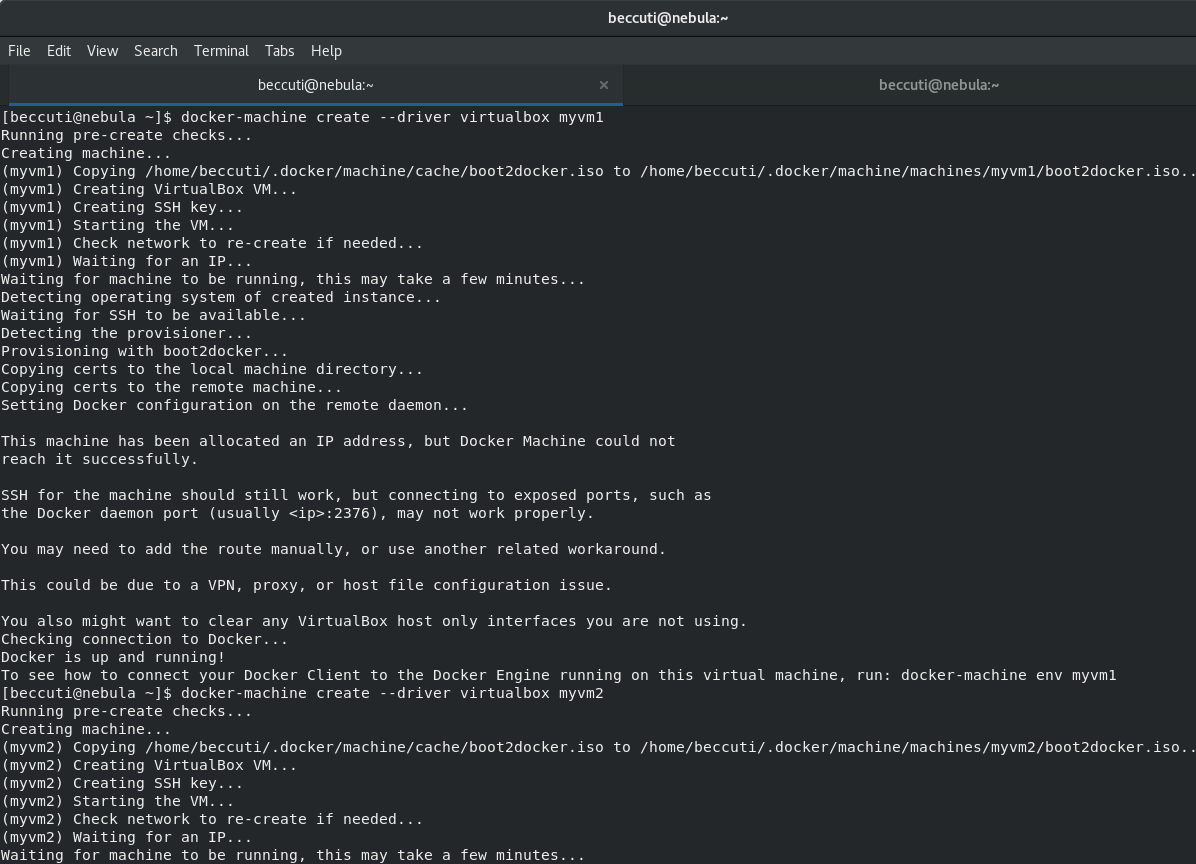
\includegraphics[width=1.00\columnwidth]{./Figure/createvm}
  		\end{center}  
 }  	  
  	

     \frame{
\frametitle{Deploy services on a cluster } 
  
 \emph{\color{PineGreen} docker-machine ls} returns the list of the created VirtualBox VMs.  \vspace{0.1cm}
     	\begin{center}
  			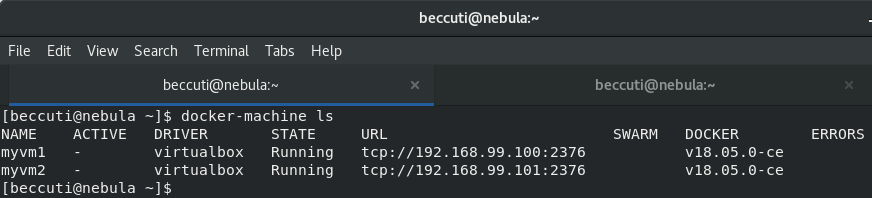
\includegraphics[width=0.90\columnwidth]{./Figure/lsvm}
  		\end{center}   
 \emph{\color{PineGreen} docker-machine stop myvm1} stops \textbf{\color{NavyBlue}myvm1} VM.  \vspace{-0.1cm}
     	\begin{center}
  			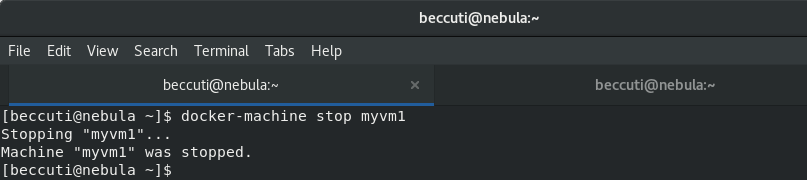
\includegraphics[width=0.90\columnwidth]{./Figure/stopvm}
  		\end{center} 
}

     \frame{
\frametitle{Deploy services on a cluster } 
    		 \emph{\color{PineGreen} docker-machine start myvm1} starts \textbf{\color{NavyBlue}myvm1} VM.  \vspace{0.3cm}
     	\begin{center}
  			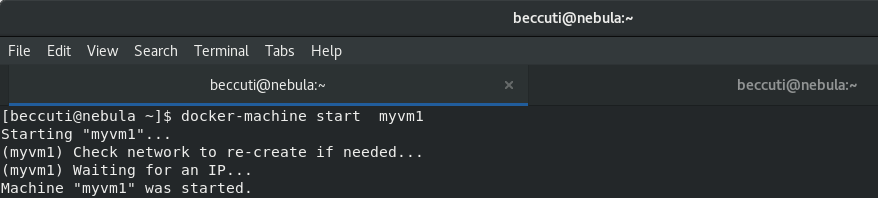
\includegraphics[width=0.90\columnwidth]{./Figure/runvm}
  		\end{center}  
 }  	    	
  
  
   \frame{
\frametitle{Deploy services on a cluster } 
  
 \emph{\color{PineGreen} docker-machine rm myvm1} removes \textbf{\color{NavyBlue}myvm1} VM.  \vspace{0.1cm}
     	\begin{center}
  			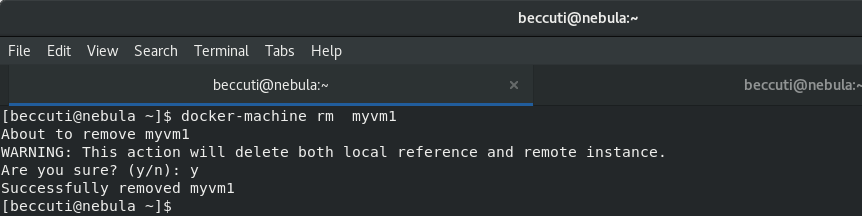
\includegraphics[width=0.90\columnwidth]{./Figure/rmvm}
  		\end{center}

 } 
 
    \frame{
\frametitle{Deploy services on a cluster } 
  
   		 \emph{\color{PineGreen} docker-machine ssh myvm1} can be used to access  \textbf{\color{NavyBlue}myvm1} VM.  \vspace{0.2cm}
     	\begin{center}
  			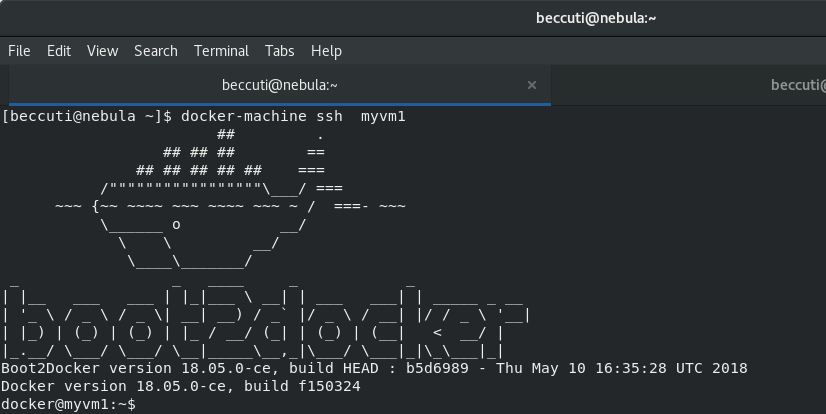
\includegraphics[width=1.0\columnwidth]{./Figure/sshvm}
  		\end{center}    
}
 
   
   \frame{
\frametitle{Deploy services on a cluster } 
   	    	  
   \emph{\color{PineGreen} docker-machine ssh myvm1 "docker ps -a"} can be used to execute commands on \textbf{\color{NavyBlue}myvm1} VM.  \vspace{0.2cm}
     	\begin{center}
  			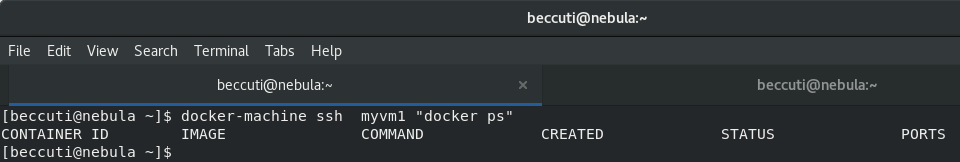
\includegraphics[width=1.00\columnwidth]{./Figure/execvm}
  		\end{center} 
  		}

   \frame{
\frametitle{Deploy services on a cluster }  
\emph{\color{PineGreen} docker-machine ssh  myvm1 "docker swarm init --advertise-addr 192.168.99.102"}  is used to initialize the swarm and set \textbf{\color{NavyBlue}myvm1} as manager.
     	\begin{center}
  			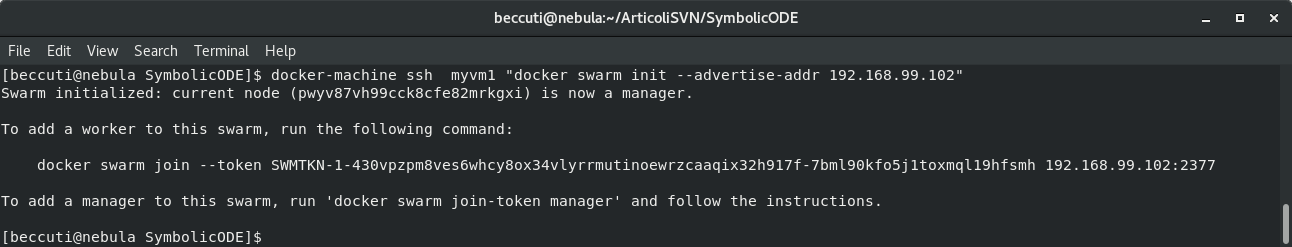
\includegraphics[width=1.00\columnwidth]{./Figure/initswarm}
  		\end{center} 
\emph{\color{PineGreen} docker-machine ssh  myvm2 "docker swarm join --token SWMTKN-1-430vpzpm8ves6whcy8ox34vlyrrmutinoewrzcaaqix32h917f-7bml90kfo5j1toxmql19hfsmh 192.168.99.102:2377"}  is used to add \textbf{\color{NavyBlue}myvm2} into the  swarm.
     	\begin{center}
  			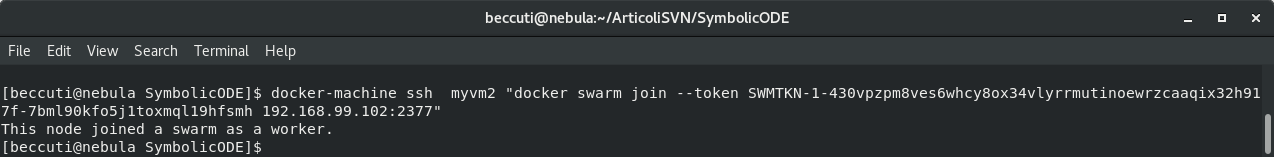
\includegraphics[width=1.00\columnwidth]{./Figure/addswarm}
  		\end{center} 

}
 
 
    \frame{
\frametitle{}
 \centerline{\Huge \color{NavyBlue} \textbf{\emph{ Deploy services}} }\vspace{0.1cm} \centerline{\Huge \color{NavyBlue} \textbf{\emph{into a Docker swarm}}}
     	\begin{center}
  			
  			
\includegraphics[width=0.40\columnwidth]{./Figure/dockerswarm}
  		\end{center} 
} 
  
   \frame{
\frametitle{Deploy services on a cluster } 
   	    	  
   \emph{\color{PineGreen} docker-machine ssh myvm1 "docker node ls"} provides information about the swarm nodes.  \vspace{-0.1cm}
     	\begin{center}
  			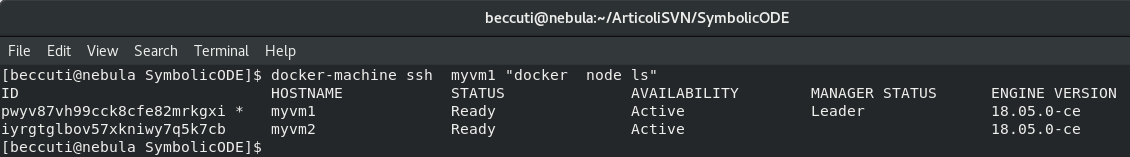
\includegraphics[width=1.0\columnwidth]{./Figure/nodelsswarm}
  		\end{center} 		
   \emph{\color{PineGreen}docker-machine ssh  myvm1 "docker node update -\;-availability drain  myvm2"} makes a node inactive.  \vspace{-0.1cm}
     	\begin{center}
  			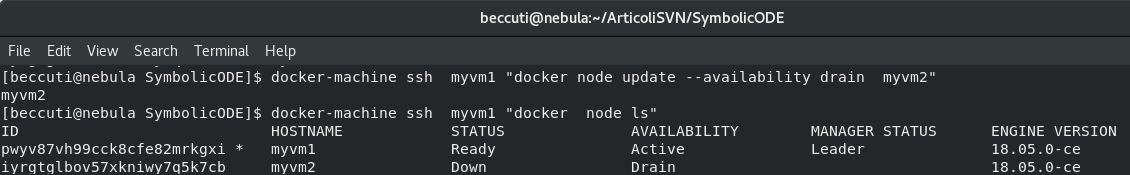
\includegraphics[width=1.0\columnwidth]{./Figure/nodeinacswarm}
  		\end{center} 
  		}   		
  	
   \frame{
\frametitle{Deploy services on a cluster } 
   	    	
   \emph{\color{PineGreen}docker-machine ssh  myvm1 "docker node update -\;-availability active  myvm2"} makes a node inactive.  \vspace{0.2cm}
     	\begin{center}
  			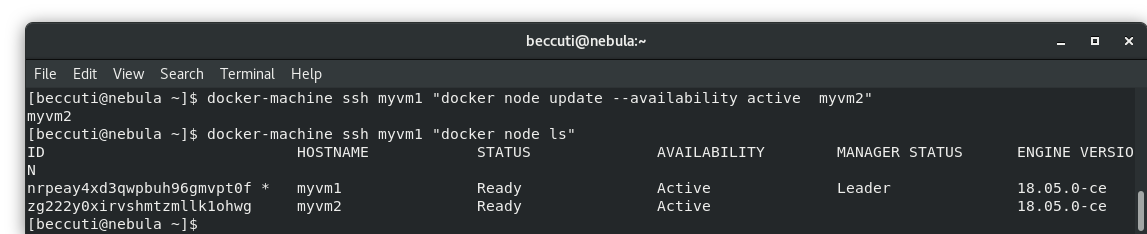
\includegraphics[width=1.0\columnwidth]{./Figure/nodeactswarm}
  		\end{center} 
  		}   	  	
  		
  	  		
  		
  	   \frame{
\frametitle{Deploy services on a cluster } 
   	    	  
   \emph{\color{PineGreen} docker-machine ssh myvm1 "docker service create   -\;-name my-web   -\;-publish published=80,target=80 -\;-replicas=1     nginx"} starts one service on a node.  \vspace{-0.1cm}
     	\begin{center}
  			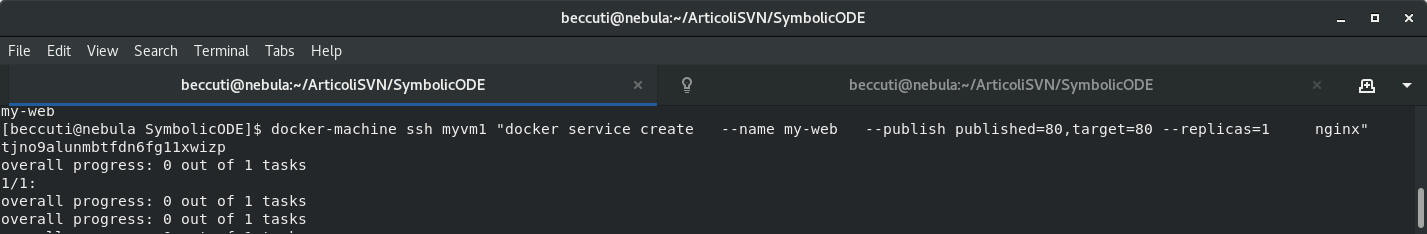
\includegraphics[width=1.00\columnwidth]{./Figure/serviceswarm}
  		\end{center} 	
  				
  \emph{\color{PineGreen}docker-machine ssh  myvm1 "docker  service ls"} and \emph{\color{PineGreen}docker-machine ssh  myvm1 "docker service  ps my-web"}
    return information on services.
    
       	\begin{center}
  			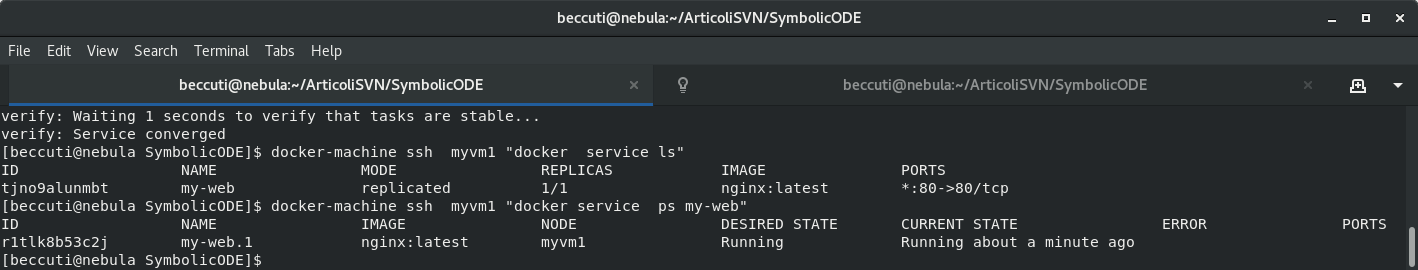
\includegraphics[width=1.00\columnwidth]{./Figure/serviceinfoswarm}
  		\end{center}  
  		}	
    		
  	   \frame{
\frametitle{Deploy services on a cluster } 
   	    	  
   \emph{\color{PineGreen}  docker-machine ssh  myvm1 "docker service scale my-web=2" 	} can be used to scale a service.  \vspace{-0.1cm}
     	\begin{center}
  			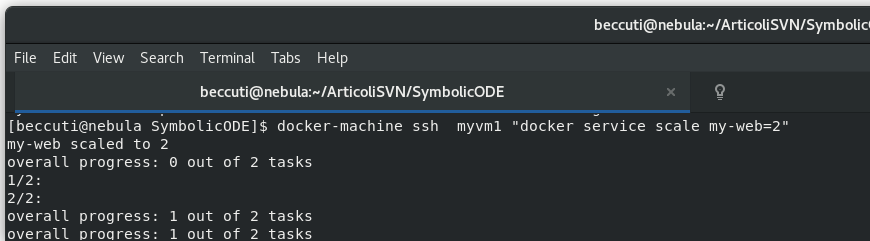
\includegraphics[width=1.0\columnwidth]{./Figure/scaleswarm}
  		\end{center} 	

       	\begin{center}
  			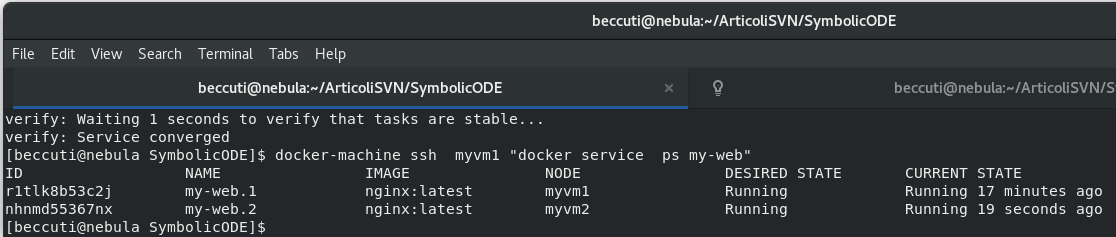
\includegraphics[width=1.0\columnwidth]{./Figure/serviceinfoswarm2}
  		\end{center}  
  		}		
  		
  	 	   \frame{
\frametitle{Deploy services on a cluster } 
   	    	  
   \emph{\color{PineGreen} docker-machine ssh  myvm1 "docker service create -\;-name my-web   -\;-publish published=80,target=80   - -mode global  nginx"
 	} can be use to automatically allocate a service on all the nodes  \vspace{-0.1cm}
     	\begin{center}
  			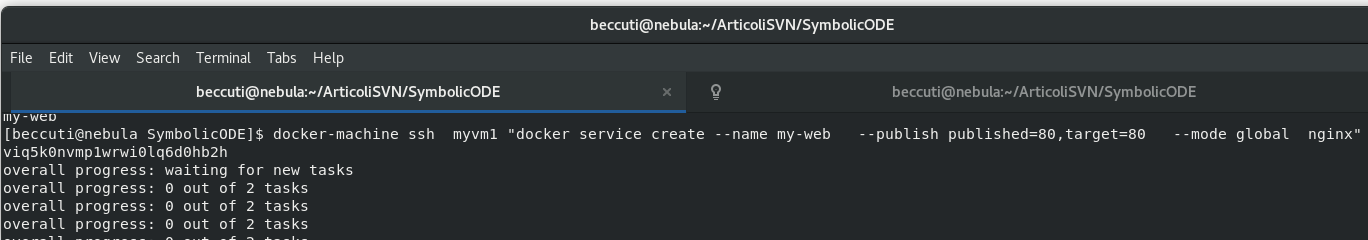
\includegraphics[width=1.0\columnwidth]{./Figure/serviceglobalswarm}
  		\end{center} 	

       	\begin{center}
  			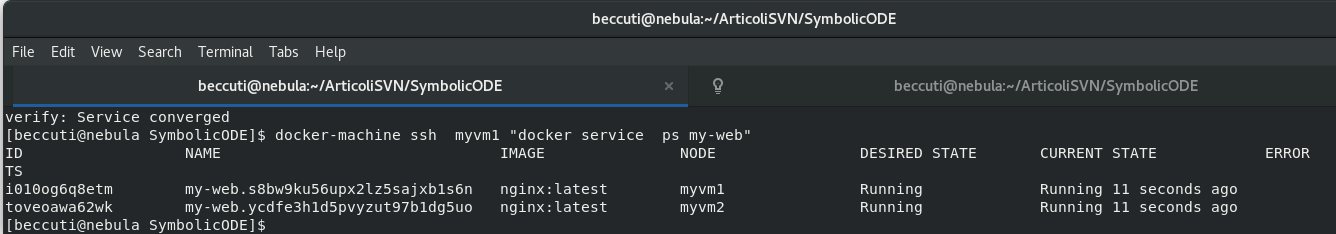
\includegraphics[width=1.0\columnwidth]{./Figure/serviceglobalswarm2}
  		\end{center}  
  		}		
	
    		
  	 	   \frame{
\frametitle{Deploy services on a cluster } 
\textbf{\color{NavyBlue}How to execute a one-shot service using swam}\vspace{0.4cm}
\begin{itemize}
\item Our goal is to use fastqc image\footnote{It must be uploaded in Docker hub} in parallel on the two nodes; \vspace{0.2cm}
\item Data can be shared using Virtualbox shared folder (i.e. \textbf{\color{NavyBlue}/hosthome}); \vspace{0.2cm}
\item We create two folders with containing fastq files. (i.e. \textbf{\color{NavyBlue}d1/} and \textbf{\color{NavyBlue}d2/});\vspace{0.2cm}
\item Option  \emph{\color{PineGreen} -\;-restart-condition=``none" } can be used for running  one-shot service;\vspace{0.2cm}
\item Option  \emph{\color{PineGreen} --mount type=bind,src=$\langle SOURCE \rangle$ ,dst= $\langle DESTINATION \rangle$} can be used for mounting the input data folder;
\end{itemize}

}		

  	 	   \frame{
\frametitle{Deploy services on a cluster } 
\textbf{\color{NavyBlue}How to execute a one-shot service using swam}\\\vspace{0.4cm}
\emph{\color{PineGreen}docker-machine  ssh   myvm1\\
\hspace{0.5cm}"docker service create -\;-replicas 1 -\;-name S1 -\;-user 1000  \\
\hspace{0.5cm}-\;-restart-condition="none"   \\
\hspace{0.5cm}-\;-mount type=bind,\\
\hspace{0.5cm}src=/hosthome/beccuti/Articoli/Presentation/DockerCorso/data/d2,\\
\hspace{0.5cm}dst=/data/scratch \\
\hspace{0.5cm}docker.io/beccuti/fastqc2   /bin/fastqc.sh"}

       	\begin{center}
  			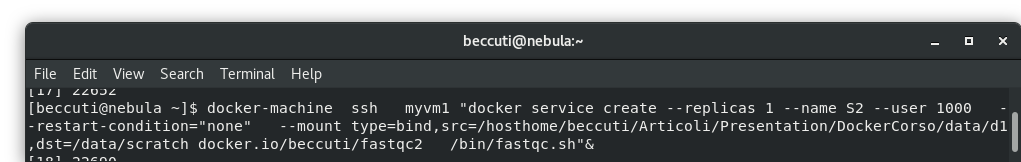
\includegraphics[width=1.0\columnwidth]{./Figure/serviceoneswarm}
  		\end{center} 

} 


 	 	   \frame{
\frametitle{Deploy services on a cluster } 
\textbf{\color{NavyBlue}How to execute a one-shot service using swam}\\\vspace{0.4cm}
\emph{\color{PineGreen}docker-machine  ssh   myvm1\\
\hspace{0.5cm}"docker service create -\;-replicas 1 -\;-name S2 -\;-user 1000  \\
\hspace{0.5cm}-\;-restart-condition="none"   \\
\hspace{0.5cm}-\;-mount type=bind,\\
\hspace{0.5cm}src=/hosthome/beccuti/Articoli/Presentation/DockerCorso/data/d1,\\
\hspace{0.5cm}dst=/data/scratch \\
\hspace{0.5cm}docker.io/beccuti/fastqc2   /bin/fastqc.sh"}

       	\begin{center}
  			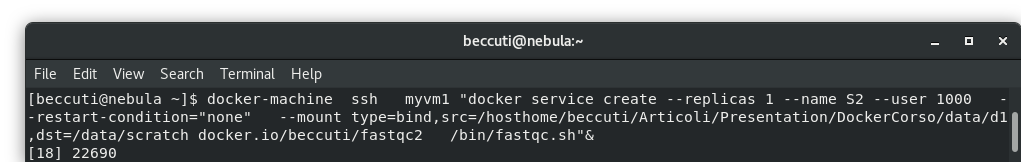
\includegraphics[width=1.0\columnwidth]{./Figure/serviceoneswarm1}
  		\end{center} 

} 


  	 	   \frame{
\frametitle{Deploy services on a cluster } 
\textbf{\color{NavyBlue}How to execute a one-shot service using swam}\vspace{0.4cm}
       	\begin{center}
  			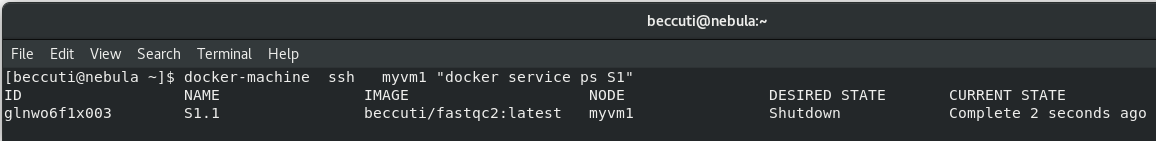
\includegraphics[width=1.0\columnwidth]{./Figure/serviceoneps}
  		\end{center} 
  		       	\begin{center}
  			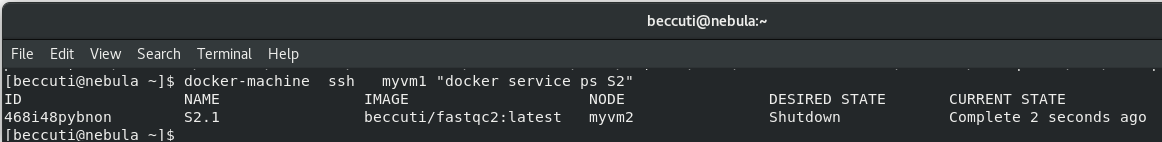
\includegraphics[width=1.0\columnwidth]{./Figure/serviceoneps1}
  		\end{center} 
}
 		